\documentclass[conference]{IEEEtran}
% *** CITATION PACKAGES ***
%\usepackage{cite}
% *** GRAPHICS RELATED PACKAGES ***
\ifCLASSINFOpdf
   \usepackage[pdftex]{graphicx}
\else
  \usepackage[dvips]{graphicx}
  \usepackage{epsfig}
\fi
\usepackage{threeparttable}
%\usepackage[cmex10]{amsmath}
\usepackage{amsmath}
\usepackage{arydshln}
\usepackage[numbers,sort&compress]{natbib}
\usepackage{float}

\begin{document}

\title{Agile Project-Based Teaching and Learning}

\author{\IEEEauthorblockN{Dagmar Monett}
\IEEEauthorblockA{Computer Science Dept.\\
Faculty of Cooperative Studies\\
%\author{\IEEEauthorblockN{\textit{(Paper submitted to SERP 2013)}}
%\IEEEauthorblockA{Dagmar Monett\\
%Computer Science Dept., Faculty of Cooperative Studies\\
Berlin School of Economics and Law, Germany\\
Dagmar.Monett-Diaz@hwr-berlin.de}}
\maketitle

%%%
% --- Abstract ---
%%%
\begin{abstract}
\boldmath
Agile courses in university settings aim to prepare students to face the ever increasing demands from the software industry, where Agile has become mainstream. This proves the teaching and understanding of Agile in such settings is of the utmost importance. This is why Agile is no longer just a part of the software engineering curriculum in Computer Science but a standalone course in most cases, though with increasing challenges for both faculty and students. This article presents yet another example case of the design, planning, development and evaluation of an agile project-based course. The reason for addressing the Agile teaching is twofold: not only are the Agile theory and practice taught and experienced in class, but also the teaching itself, and consequently the learning, has been adapted to changing requirements and priorities in each edition of the course. Making it project-based allows students to work with realistic projects through which they learn Agile more effectively, in collaborative and self-organizing teams. These insights, as well as settings and experiences over a total of 4 years, are addressed in this article.
\end{abstract}

%%%
% --- Keywords ---
%%%
\begin{keywords}
Agile, eXtreme Programming, teaching, project-based learning.
\end{keywords}

%%%
% --- Introduction ---
%%%
\section{Introduction}
\label{sec:intro}

There are lots of strong reasons for including Agile principles in CS education \cite{HaDu07}. Positive experiences that go from \textit{project-based} Computer Science (CS) courses using Agile \cite{Pe09,Scetal12} over \textit{Agile teaching} \cite{RaAn06} to \textit{Agile instructional design} \cite{LeVa12} have had a common denominator: the practices, the values and the methods of the agile software development are essential; Agile is a current mainstream in the software industry \cite{VO13} and educational environments are profiting from this, too. Meanwhile, project-based learning has proven to be very attractive in tertiary teaching: students learn the discipline via a realistic project, they pursue questions and connect them to activities that are part of the project, they construct knowledge and autonomously work towards a final product, as well as they master the curriculum standards with academic rigor \cite{Th00}.

The module \textit{Project Management} is part of the CS education during the third semester at the Berlin School of Economics and Law (BSEL). By successfully passing this module, dual studies CS students can obtain 14 ECTS-credits,\footnote{European Credit Transfer and Accumulation System. One credit point is equivalent to 30 hours of study.} which are assigned by considering the following proportion: a 20\% of them goes to the sub-module \textit{Project and Quality Management}, a 30\% goes to the sub-module \textit{Multidisciplinary Lab using Agile techniques}, and a 50\% goes to the sub-module \textit{Practice Transfer}, where students are at their enterprises and where they should apply gained knowledge in software engineering in general and in Agile and project management in particular. Credit hours, however, were never intended to be a measure of student learning, as Laitinen argues in \cite{La13}. She brings forward the argument that there should be found ``what students are expected to --and actually do-- learn'', as well as the measurements to meaningfully assess what they have learned, not only concerning time-based units. By introducing Agile project-based techniques in CS assignments and by accurately defining both the learning goals and their evaluation forms, as it is further presented in this article, a positive step in this direction is achieved. 

Much of the Agile courses in university settings have a common goal: to prepare students to face the ever increasing challenges in the software industry. Jaccheri and Morasca define in \cite{JaMo06} five main roles that industry can play in software engineering education from the point of view of the university teacher: industry as students, as teachers, as researchers, as customers, and as former students. Three of these roles are well-identified in the mentioned module \textit{Project Management}:

\begin{itemize}
  \item Industry as teachers: the sub-module \textit{Project and Quality Management} runs parallel to the sub-module \textit{Multidisciplinary Lab using Agile techniques}. The first sub-module is taught by an industry specialist in close collaboration with the latter's teacher.
  \item Industry as customers: a real customer, who presents a problem to the students and who is available for consulting, is simulated in the Lab, if it is not possible to invite ``a real'' one. The concrete problem that is selected and the algorithm for solving it are also present in many industrial applications.
  \item Industry as former students: there are a Faculty Technical Commission and a Faculty Commission for Cooperative Studies at the BSEL both integrated by several industry partners, former dual studies students some of them, that discuss and approve the curriculum and other teaching and learning issues. Part of the faculty is composed of former BSEL students as well.
\end{itemize}

Two of the most important advantages of the program that prepare CS students for their further professional life are: firstly, students from the Faculty of Cooperative Studies are dual studies students and work in German companies from their first career's semester on. This means, they gain practical experience in real industry scenarios from the beginning of their studies on. Second, the sub-module \textit{Multidisciplinary Lab using Agile techniques} (Lab using Agile, for short) provides them with several hard skills like specifying, designing, implementing and testing software, as well as communicating, presenting, and working in a team, to name a few soft skills. Furthermore, both advantages successfully minimize new hires' common frustrations, as addressed in \cite{Co02}. 

The Lab using Agile uses an interdisciplinary approach from the viewpoint of different cross-disciplinary topics addressed there. Perhaps these are reasons why the course has been favorably received by both faculty and students. Its careful design and planning, as well as its constant adaption to changing teaching and learning requirements has proven extremely effective in project-based courses. The remainder of this paper describes aspects for the Lab using Agile in detail.


%%%
% --- Agile and XP techniques ---
%%%
\section{Agile and XP techniques}
\label{sec:agileXP}

One of Agile's most used methodologies is eXtreme Programming (XP), which has also been very popular in CS teaching \cite{Go04,KeDi04,MuTi01,ShWi02,StLuEr08}. For example, Stapel and colleagues propose in \cite{StLuEr08} a XP lab design property system for teaching a project-based XP course to CS master students, emphasizing in XP practices as part of a closed block course. Their work inspired the study summarized in this paper, which recommends a change from a weekly course to a blocked one. However, not only the course design, its type and the students' level, but also the blocks' duration, the XP iteration lengths, the team sizes, and the project content, among others indicators, differentiate their research from the one presented in this paper. Valuable insights from other works evaluating Agile in education environments also influence the findings presented here.

Pair programming is no longer extrinsic to CS education. In \cite{MeVaGo08}, for example, a case study concludes that pair programming is an effective approach for mastering computer programming together with cooperative learning principles. The authors extensively review the literature about the advantages and disadvantages of pair programming as a teaching-learning strategy, too. In \cite{XuRa05}, the authors additionally comment about the benefits of pair programming when practicing it in graduate software engineering class projects. Furthermore, several works have been published concerning both the strengths and weaknesses of pair programming but from the perspective of the Agile community.

The rest of the XP techniques are also introduced to the students in the Lab using Agile, both theoretical and practically. The students are, however, undergraduate students with little programming experience. In fact, they have only attended a few semesters at the university. Nevertheless, they learn quickly how to develop software with the aid of Agile, they solve a concrete real problem working in teams and they gain experiences by simulating a working day at an enterprise as part of the course project. 

Differentiated supervision and guidance allow for better reactions to problems that might arise when introducing Agile or simply when working with others. In the Lab using Agile, individual and general coaching is offered as well. The faculty coaches individuals and teams in the course and is able to monitor progress and development anytime. Thus, continuous feedback can be provided to the students, to the teams and to the entire group. In reciprocation, students should be capable of presenting different stages of working software, and they should discuss with faculty in the role of (simulated) customers, acceptance criteria for their software products. In the coaching sections, it is expected that students come with concrete questions they have prepared in advance about any topic they need advice on.

\begin{table}[!t]
  %% increase table row spacing, adjust to taste
  \renewcommand{\arraystretch}{1.3}
  \setlength{\tabcolsep}{0.6em}
  \caption{Course schedule: teaching blocks and semester credit hours.}
  \label{tab:SCHblocks}
  \centering
  \begin{tabular}{|c|cc|cc|c|}
    \hline
    \bfseries Block 1 & \multicolumn{2}{|c|}{\bfseries Block 2} & \multicolumn{2}{|c|}{\bfseries Block 3} & \bfseries Block 4\\
    \hline
    \textit{Day 1} & \multicolumn{1}{|c|}{\textit{Day 2}} & \textit{Day 3} & \multicolumn{1}{|c|}{\textit{Day 4}} & \textit{Day 5} & \textit{Day 6}\\
    \hline
    \hline
    & \multicolumn{1}{|c|}{8 SCH} & \multicolumn{1}{|c|}{8 SCH} & \multicolumn{1}{|c|}{8 SCH} & \multicolumn{1}{|c|}{8 SCH} & \\
    6 SCH & \multicolumn{1}{|c|}{(PC Lab)} & \multicolumn{1}{|c|}{(PC Lab)} & \multicolumn{1}{|c|}{(PC Lab)} & \multicolumn{1}{|c|}{(PC Lab)} & 6 SCH \\
    \cline{2-4}
    \cline{4-5}
    & \multicolumn{2}{|c|}{16 SCH} & \multicolumn{2}{|c|}{16 SCH} & \\
    \hline
    \hline
    \multicolumn{6}{|c|}{44 SCH} \\
    \hline
\end{tabular}
\end{table} 




%%%
% --- Course Schedule ---
%%%
\section{Course Schedule}
\label{sec:courseschedule}

Table \ref{tab:SCHblocks} shows the course schedule for the Lab using Agile in teaching blocks and semester credit hours (SCH, 1 SCH meaning what follows 45 minutes of teaching time). The course is divided into four teaching blocks for a total of 44 SCH. Blocks 2 and 3 take place in a PC Lab. They are mainly intended for teamwork. In the Fall 2009 and 2010 editions of the course, three XP iterations were programmed for respective three product releases. However, in the Fall 2011 and 2012, only two XP iterations and their respective releases were planned, in response to the course appraisals administered at the end of the previous terms. More on this respect can be found in Section \ref{sec:teacheval}.

Table \ref{tab:Agileblocks} shows the same course schedule but in teaching blocks and Agile cycles. Both \textit{Syllabus} and \textit{Intro I} at Day 1 conform Block 1 and refer to an introductory section, which states the purpose and goals of the course, as well as the theory about the algorithms selected to solve the customer problem. \textit{Intro II} at Day 2 refers to an introduction to Agile and to XP. Days 2 and 3 are two continuous calendar days from Block 2, as well as days 4 and 5 are from Block 3. \textit{Iteration 1} starts with \textit{Planing game 1} and takes between three and four weeks until \textit{Release 1} is accomplished, with only the first two days at the university. This similarly occurs for \textit{Iteration 2}, whose \textit{Release 2} takes place at the end of the course, at Day 6. The \textit{Conclusions} are mainly based on the presentations of the final product releases and on the teacher's feedback concerning the projects as a whole. In \cite{StLuEr08}, to name one crucial difference to this work, the block course has no interruption at all: the (very short) iterations are continuously located in the course time frame.

\begin{table}[!t]
  %% increase table row spacing, adjust to taste
  \renewcommand{\arraystretch}{1.3}
  \setlength{\tabcolsep}{0.6em}
  \caption{Course schedule: teaching blocks and Agile cycles.}
  \label{tab:Agileblocks}
  \centering
  \begin{tabular}{|c|cc|cc|c|}
    \hline
    \bfseries Block 1 & \multicolumn{2}{|c|}{\bfseries Block 2} & \multicolumn{2}{|c|}{\bfseries Block 3} & \bfseries Block 4\\
    \hline
    \textit{Day 1} & \multicolumn{1}{|c|}{\textit{Day 2}} & \textit{Day 3} & \multicolumn{1}{|c|}{\textit{Day 4}} & \textit{Day 5} & \textit{Day 6}\\
    \hline
    \hline
    & \multicolumn{1}{|c|}{Intro II} &  & \multicolumn{1}{|c|}{Release 1} &  & \\
    Syllabus & \multicolumn{1}{|c|}{Planing game 1} &  & \multicolumn{1}{|c|}{Planing game 2} &  & Release 2 \\
    \cline{2-2}
    \cline{4-4}
    Intro I & \multicolumn{2}{|c|}{Iteration 1} & \multicolumn{2}{|c|}{Iteration 2} & Conclusion \\
    & \multicolumn{2}{|c|}{(Incremental teamwork)} & \multicolumn{2}{|c|}{(Incremental teamwork)} & \\
    \hline
\end{tabular}
\end{table}

\textit{Incremental teamwork} in blocks 2 and 3 means students become more independent while working in a team. Students not only do work incrementally on different tasks without interruption while planning and developing software: they also apply Agile techniques that make them more independent. They progressively need lesser coaching from faculty for mastering activities that are more complex with time. In order to cope with these challenges, the course schedule includes more time for programming and less for other didactic exercises, also in a progressive way.


%%%
% --- Learning and Teaching Goals ---
%%%
\section{Learning and Teaching Goals}
\label{sec:coursegoals}

Faculty should be aware of both the coarse and the fine-grained learning goals for a course, in order to break down those goals and to focus on the content to be taught. The former, the coarse-grained learning goals, are often defined in the curriculum in a general way. The latter ones help faculty to plan and to draw up in detail what students need to master and the ways of achieving and evaluating that. By defining thoroughly the fine-grained learning goals of the Lab using Agile, faculty creates the course syllabus without difficulty, and individual blocks and days are planed easier. This does not require a straightforward, additional effort for the conception of all these teaching materials, but the time saved later pays dearly the invested one.

The second block of the Lab using Agile is dedicated to the first experiences with the XP practice, especially at Day 2. The fine-grained learning goals of the second block (B2) for the firsts double credit hours (2 SCH each, i.e., 1$\frac{1}{2}$ hours) are: 

\textit{After completion of the second block, the students will be able$\dots$ }

\textit{\bfseries B2.1 (2 SCH):} $\dots$\textit{to identify and to describe software requirements using story cards; to assess their priorities; to coordinate and to discuss their inclusion in the current iteration; and to plan and to schedule related activities for the first XP iteration.}

\textit{\bfseries B2.2 (2 SCH):} $\dots$\textit{to meet and to participate in ``stand-ups'' or daily meetings; to develop software programming in pairs.}

\textit{\bfseries B2.3 (2 SCH):} $\dots$\textit{to discuss and to formulate rules for working in a team; to discuss and to formulate rules for the work of several teams in a room.}

\textit{\bfseries B2.4 (2 SCH):} $\dots$\textit{to develop software working in teams.}

Didactic exercises worked out in this block include organizational aspects that allow for better collaborative work when applying XP, since this is essential to Agile \cite{Beetal01}. Rules for working in a team are then to be discussed by the students, for example, and each project group could present its set of rules using a flip chart in one of the sessions.

\textit{Teaching screenplays} were used to better schedule the sequence of concrete teaching and learning activities to be included into a class, as well as the time required to complete them. They were planned using a sandwich structure, i.e., by combining passive and active learning units, and are like lesson plans or teaching worksheets that describe the teaching roadmap for a class or for part of a class in detail. For example, the teaching screenplay for the first double credit hour from block B2 is shown in Table \ref{tab:screenplay1}. It corresponds to the fine-grained learning goals defined above for the first double credit hour of that block, i.e., for B2.1.

\begin{table}[!t]
  %% increase table row spacing, adjust to taste
  \renewcommand{\arraystretch}{1.3}
  \setlength{\tabcolsep}{0.6em}
  \caption{Example teaching screenplay for the double credit hour B2.1.}
  \label{tab:screenplay1}
  \centering
  \begin{tabular}{|c|c|c|l|}
    \hline
         &                  & 5    & \textbf{Start} -- \textit{passive unit} \\
         & \textbf{Entry}   & min. & \hspace{0.5em} Welcoming (oral) \\
         &                  &      & \hspace{0.5em} Contents and time schedule (flip chart) \\
    \cline{2-4}
         &                  &      & \textbf{Content 1} -- \textit{passive unit} \\
         &                  & 20   & \hspace{0.5em} Motivation (oral) \\
         &                  & min. & \hspace{0.5em} Learning goals (flip chart) \\
         &                  &      & \hspace{0.5em} Planning game (flip chart, blackboard) \\
         &                  &      & \hspace{0.5em} Story cards (blackboard)\\
    \cline{3-4}
         &                  & 3    & \textbf{Brainstorming} -- \textit{active unit} \\
         &                  & min. & \hspace{0.5em} Collect examples (plenum) \\
    \cline{3-4}
         &                  &      & \textbf{Content 2} -- \textit{passive unit} \\
    90   & \textbf{Working} & 20   & \hspace{0.5em} Project description (hand outs) \\
    min. & \textbf{phase}   & min. & \hspace{0.5em} Project goals (blackboard) \\
         &                  &      & \hspace{0.5em} Project requirements (hand outs) \\
         &                  &      & \hspace{0.5em} Requirements for 1st release (blackboard) \\
    \cline{3-4}
         &                  & 2    & \textbf{Introduce exercise} -- \textit{passive unit} \\
         &                  & min. & \hspace{0.5em} Planning game: method, time management (oral) \\
    \cline{3-4}
         &                  &      & \textbf{Knowledge transfer} -- \textit{active unit} \\
         &                  & 35   & \hspace{0.5em} Planning game 1st iteration (teamwork, coaching) \\
         &                  & min. & \hspace{1em} Define story cards \\
         &                  &      & \hspace{1em} Set priorities \\
         &                  &      & \hspace{1em} Discuss realization \\
    \cline{2-4}
         &                  &      & \textbf{End} -- \textit{active and passive unit}\\
         & \textbf{Exit}    & 5    & \hspace{0.5em} Questions, feedback (oral) \\
         &                  & min. & \hspace{0.5em} Conclusions (oral) \\
         &                  &      & \hspace{0.5em} Short about the next double SCH, i.e., B2.2 (oral) \\
    \cline{1-4}
\end{tabular}
\end{table}

19 such teaching screenplays are needed for blocks 1 to 3, i.e., one screenplay as in Table \ref{tab:screenplay1} for each double SCH. However, much of them are only an outline like the one presented in Table \ref{tab:screenplay2}. All teaching screenplays can be adjusted and adapted depending on the concrete class' rhythm when developing the course projects, which is just an expression of the Agile project-based teaching. An extra column could be added to the screenplays, too, for comments on self reflection and on self assessment after completing the scheduled exercises and activities.


%%%
% --- Project Requirements ---
%%%
\section{Project Requirements}
\label{sec:projreq}

The general project description was formulated as follows: \textit{Solve the traveling salesman problem (TSP) using a metaheuristic algorithm in the context of an XP project. Wanted is a software product with a graphical user interface (GUI) that includes menus and controls to define settings and that visualize results, as well as with a graphical window to show both the cities and the optimization process in real time.}

\begin{table}[!t]
  %% increase table row spacing, adjust to taste
  \renewcommand{\arraystretch}{1.3}
  \setlength{\tabcolsep}{0.6em}
  \caption{Example teaching screenplay for a double credit hour with teamwork.}
  \label{tab:screenplay2}
  \centering
  \begin{tabular}{|c|c|c|l|}
    \hline
         &                  & 2    & \textbf{Start} -- \textit{passive unit} \\
         & \textbf{Entry}   & min. & \hspace{0.5em} Welcoming (oral) \\
         &                  &      & \hspace{0.5em} Goals and time schedule (flip chart) \\
    \cline{2-4}
         &                  &      & \textbf{Teamwork and coaching} -- \textit{active unit} \\
    90   & \textbf{Working} & 83   & \hspace{0.5em} Incremental software development (by students) \\
    min. & \textbf{phase}   & min. & \hspace{0.5em} Individual team coaching (by faculty) \\
         &                  &      & \hspace{0.5em} Questions, feedback (team-oriented) \\
    \cline{2-4}
         &                  & 5    & \textbf{End} -- \textit{passive unit}\\
         & \textbf{Exit}    & min. & \hspace{0.5em} Conclusions (oral) \\
         &                  &      & \hspace{0.5em} Short about the next double SCH (oral) \\
    \cline{1-4}
\end{tabular}
\end{table}

Students should use metaheuristics algorithms, like genetic algorithms (GA) and ant colony systems (ACO), to solve instances of the TSP. They should test their programs using 2-dimensional, symmetric TSP instances of geographical problems from TSPLIB \cite{Re91}, as well as they should report both their findings and the software development using Agile in a research paper of at least five pages, following the guidelines for two-column conference proceeding in IEEE style. 

Software requirements are defined by the customer (real or simulated) at the beginning of each XP iteration, depending on the focus the software development in that phase is centered around. Only those requirements related to the GUI development, for instance, are defined, specified, planned, and prioritized in the same planning game. Those requirements concerning the data and the algorithms to process them are defined in another planning game. Whether to start with the GUI or with the logic was discussed with the students. For many of them it was more important and attractive to have a working product with options and other components to present to the customer in the different releases, into which other functionalities could be added onto.

In Fall 2012, the first release, at the beginning of the third block (see Table \ref{tab:Agileblocks}), was an ``individual'' meeting of each team with faculty playing the roles of \textit{customer} and \textit{coach}. The second release, in the last course's block, was a ``public'' meeting (all teams, in plenum), where faculty played both the \textit{customer} and the \textit{evaluator} roles. Each team presented a software prototype in the former, as well as it addressed the main aspects related to other Agile methods and techniques. In the latter, the final release, a formal oral presentation of about 35 minutes gave insights about the final product, about the project development, and about the experiences and lessons learned during the project completion.

Emphasis was also put on project management tools for collaborative work. The students had the opportunity, at least in the last two editions of the Lab using Agile, to test and to use several new tools (for them), like Redmine\footnote{Redmine (at http://redmine.org) is a project management web application.} and Trello\footnote{Trello is a board-based collaboration tool. See more at http://trello.com/.}, for instance. 


%%%
% --- Course Evaluation ---
%%%
\section{Course Evaluation}
\label{sec:courseeval}

The composition and the size of the class, together with other information related to the last four editions of the course, are presented in Table \ref{tab:groupsize}. The number of students answering a customized, anonymous questionnaire at the end of the semester is given in parenthesis for each course edition. 

In the Falls 2009 and 2010, the course was offered weekly and there were a total of three XP iterations (and therefore, a total of three releases). No special didactic methods were applied at that time. In each of both editions, a different algorithm was considered to solve the TSP problems, i.e., ACO in Fall 2009 and GA in 2010. Students had difficulties especially when programming in the class, since the time available each week was minimal. They also had problems that prevented them completing their projects on time.

\begin{table}[!t]
  %% increase table row spacing, adjust to taste
  \renewcommand{\arraystretch}{1.3}
  \setlength{\tabcolsep}{0.6em}
  \caption{Characteristics of the last four course editions.}
  \label{tab:groupsize}
  \centering
  \begin{tabular}{|l|c|c|c|c|c|c|c|}
    \hline
    & \bfseries Group & \bfseries Female & \bfseries Weekly$/$ & \bfseries Agile & \bfseries Algo- & \bfseries Special & \bfseries Special\\
    \bfseries Fall & \bfseries size & \bfseries prop. & \bfseries Blocks & \bfseries iter. & \bfseries rithm & \bfseries didactic & \bfseries coaching\\
    \hline \hline
    2009 & 30(30) & 1  & w & 3 & ACO & -- & -- \\
    2010 & 30(30) & 2  & w & 3 & GA  & -- & -- \\
    2011 & 24(24) & -- & b & 2 & ACO & ++ & + \\
    2012 & 28(19) & 2  & b & 2 & ACO & ++ & ++ \\
    \hline
  \end{tabular}
\end{table}

In the Falls 2011 and 2012, however, the course was divided in four presence blocks, as it is presented in Table \ref{tab:SCHblocks}. Both editions of the course scheduled only two XP iterations, as derived from students' feedback in the former courses. The algorithm used for solving TSP was the same in both cases (i.e., ACO). Both editions included several special didactic methods not applied before, as well as a close team coaching by the professor, more intensive in Fall 2012. Additionally, the faculty was coached in Fall 2012 by an external training coach,  expert in didactic in higher education.


%%%
% --- Evaluating Students ---
%%%
\subsection{Evaluating Learning}
\label{sec:learneval}

Each student can earn at most 100 points, which are then converted to a grade-point system in the German grading scale, as usual. A final student's grade is the team grade to which they belong. It is determined using a percentage system with 20\% for each of the following areas: first release, second release, research paper, software program, and project management. 

For assessing the releases and the team presentations, an evaluation form was designed by the faculty. It considers key components like presentation skills, content, timing, confidence, quality, and so on. The research paper was evaluated according to guidelines for scientific events. What to consider for both its content and structure was previously discussed with the students. Last but not least, the software program should satisfy all requirements, the teams should submit an executable version out of bugs, and the main software features and their functioning should be shown in the final presentation, without forgetting the project management aspects related to the project as a whole.
 

%%%
% --- Evaluating Teaching ---
%%%
\subsection{Evaluating (not only) Teaching}
\label{sec:teacheval}

By the term's end, a questionnaire independent of formal faculty evaluations was administered to students. The questions catalogue with their descriptive scale values is shown in Table \ref{tab:questions}. The questions are grouped in four major topics, these corresponding to the course requirements in particular, to teaching in general, to how students learned, and to Agile. 

\begin{table*}[!t]
  %% increase table row spacing, adjust to taste
  \renewcommand{\arraystretch}{1.3}
  \setlength{\tabcolsep}{0.6em}
  \caption{Questions catalogue with descriptive scale values.}
  \label{tab:questions}
  \centering
  \begin{threeparttable}
  \begin{tabular}{|c|l||cccc|}
    \hline
    & & \multicolumn{4}{|c|}{\bfseries Descriptive scale values and index}\\
    \cline{3-6}
    \multicolumn{1}{|c|}{\bfseries Id.} & \multicolumn{1}{|l||}{\bfseries Question} & \multicolumn{1}{|c}{4} & \multicolumn{1}{c}{3} & \multicolumn{1}{c}{2} & \multicolumn{1}{c|}{1\tnote{a}}\\
    \hline\hline
    A & What do you think about the required time for the course & too high & normal & too low & abstention\\
    B & How were the requirements concerning the course assignments/tasks? & too high & realistic & too low & abstention\\
    C & How did you find the problem that was selected to be solved (i.e. TSP)? & motivating & neutral & dissuasive & abstention\\
    D & How did you find the algorithm that was selected to solve the user problem? & motivating & neutral & dissuasive & abstention\\
    \hline
    E & How was the introduction on the course goals and topics? & very good & normal & very bad & abstention\\
    F & How did the teacher/on-site customer respond to the questions, how was her feedback? & very good & normal & very bad & abstention\\
    \hline
    G & Do you feel as if you would have learned something during the course? & very much & normal & very little & abstention\\
    H & How did the course form your interest on the working field? & motivating & neutral & dissuasive & abstention\\
    \hline
    I & Did you enjoy Agile practices, especially XP? & very much & normal & very little & abstention\\
    J & Do you think you have improved your programming skills when participating in the XP project? & very much & normal & very little & abstention\\
    K & And how about your social skills? Did you improve them? & very much & normal & very little & abstention\\
    L & Do you think that using XP improves the productivity of small teams? & very much & normal & very little & abstention\\
    M & Do you think that using XP improves the quality of the code? & very much & normal & very little & abstention\\
    N & Do you think that Pair Programming speeds up the developing process? & very much & normal & very little & abstention\\
    O & How did you find the planning game at the beginning of each iteration? & very helpful & normal & irritating & abstention\\
    \hdashline
    P & How was the division in two (Fall 2011, Fall SS2012) / three (Fall 2009, Fall 2010) releases? & excessive & adequate & insufficient & abstention\\
\hline
\end{tabular}
\begin{tablenotes}
  \item[a] The scale index with value 1 is reserved for abstentions, for each question, so that students can leave questions unanswered.
\end{tablenotes}
\end{threeparttable}
\end{table*}

Students could also provide an overall evaluation of the course, including what they liked the most, what they did not like at all, as well as further suggestions and comments.


%%%
% --- Results ---
%%%
\section{Results and discussion}
\label{sec:results}

Figure \ref{fig:polargraph} shows a polar line chart with an area layer divided in four sectors that depend on the four general questionnaire topics mentioned so far. The question P is not included since it refers to different scenarios (two or three releases).

\begin{figure}[!t]
\centering
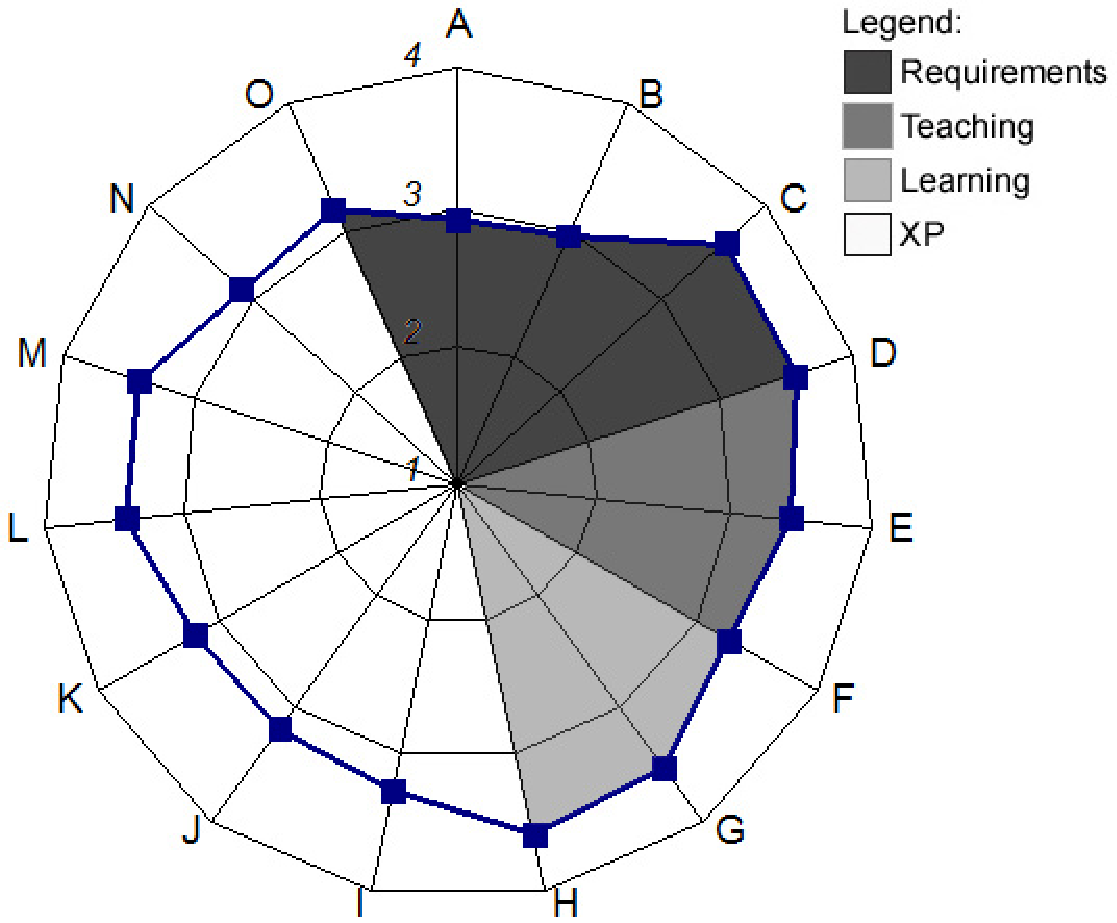
\includegraphics[width=6.2cm]{Resources/webgraph.pdf}
\caption{Questionnaire results averaged for the four editions of the course.}
\label{fig:polargraph}
\end{figure}

The plotted data are computed using the following formula, which represents a weighted average for each question $i$:
\begin{align*}
y &= \frac{\sum\limits_{j=1}^4 (5-j) \cdot v_{ij}}{N}\\
&= \frac{4 \cdot v_{i1} + 3 \cdot v_{i2} + 2 \cdot v_{i3} + v_{i4}}{103}
\end{align*}
$N$ being the total number of students responses over the four years ($N=103$) and $v_{ij}$ being the sum of all responses multiplied by a scaling of the descriptive scale value $j$, for each question. For example, question A refers to the required time for the course and it has the descriptive scale values \textit{too high}, \textit{normal}, \textit{too low}, and \textit{abstention} (see Table \ref{tab:questions}). The number of total responses were 13, 70, 18, and 2 for each descriptive value, respectively. Thus, $y=2.9126$ in the polar line chart for question A, which means that a substantial number of all students considered the required time as normal.

The rest of the plotted data can be read in a similar way: most students found the requirements concerning the course assignments (question B) to be realistic, the TSP and solving it with the selected metaheuristic (questions C and D) were motivating, and so on. All in all, the students' feedback was very positive in general, particularly regarding Agile.

Figure \ref{fig:11vs12} shows a polar line chart with a polar area layer and a polar line layer comparing in detail some data for the Fall 2011 and for the Fall 2012, respectively. Only the questionnaire topics ``how students learned'' and ``Agile techniques'' are considered. In the figure, \textit{Learning} refers to the question with identifier \textit{G}, \textit{Interest in the field} to \textit{H}, \textit{Enjoy Agile} to \textit{I}, \textit{Programming skills} to \textit{J}, \textit{Social skills} to \textit{K}, \textit{Productivity small teams} to \textit{L}, \textit{Code quality} to \textit{M}, \textit{Development} to \textit{N}, \textit{Planning game} to \textit{O}, and \textit{Two releases} to \textit{P}, respectively, as specified in Table \ref{tab:questions}. The corresponding values are listed in Table \ref{tab:t11vs12}, which includes the relative percentage of responses for each descriptive scale value, for each question, not including the abstentions for being irrelevant. Such details give more information than the weighted average when comparing both courses.

\begin{figure}[!t]
\centering
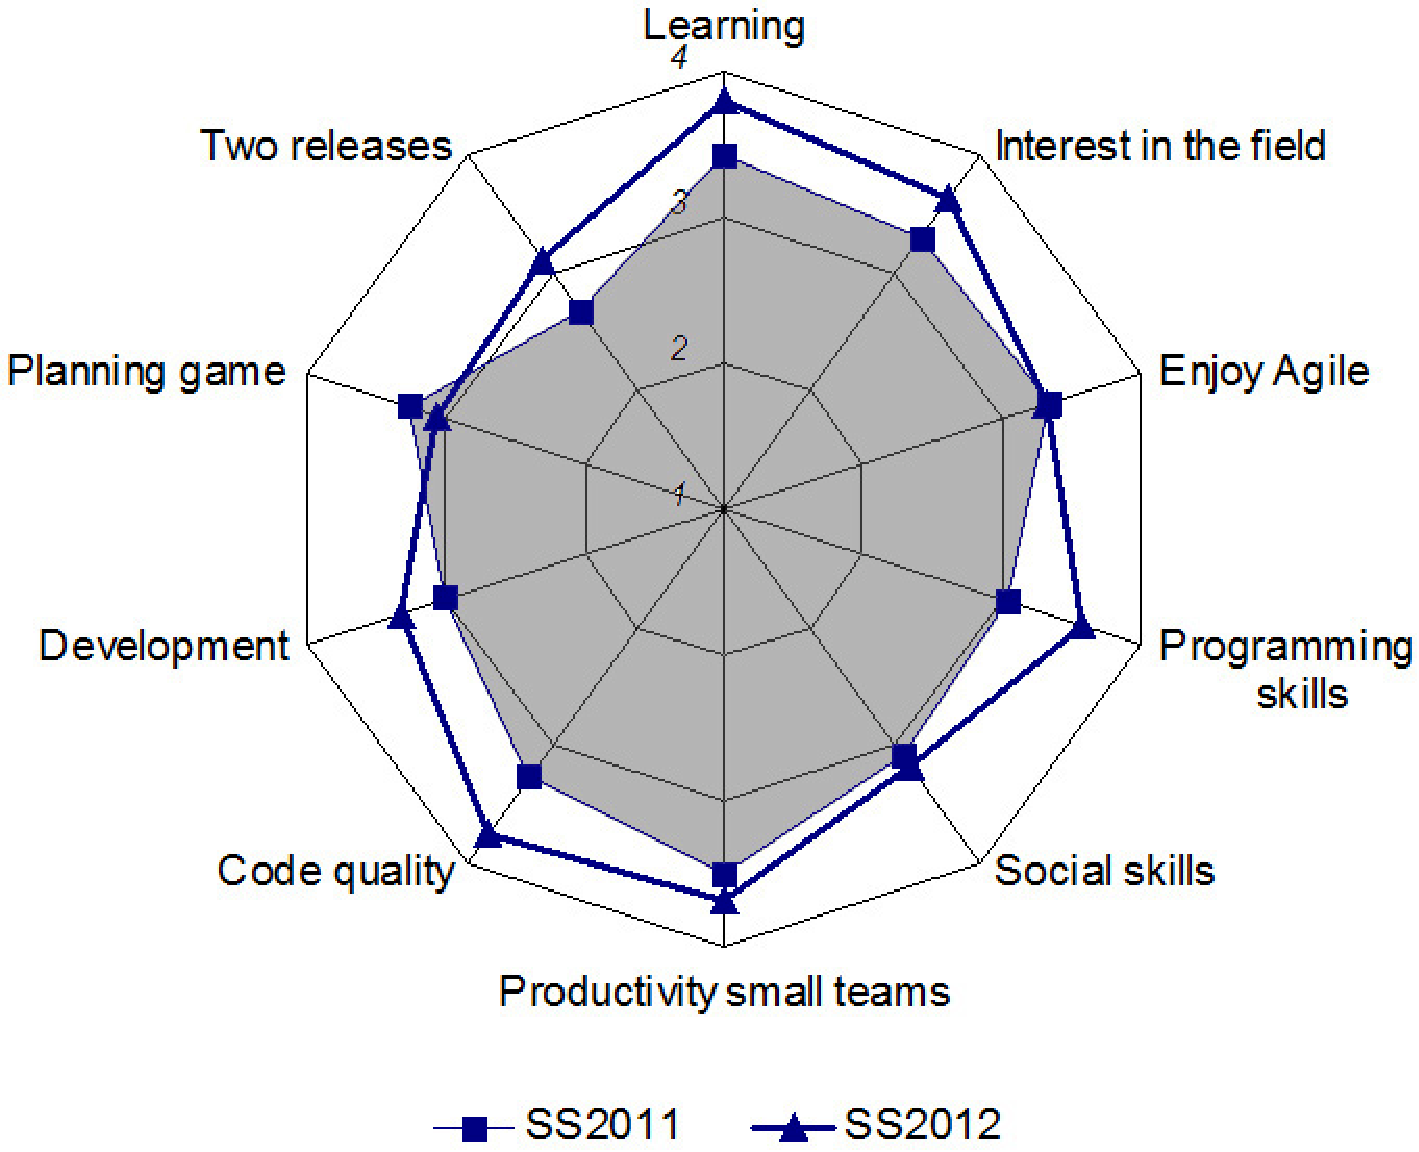
\includegraphics[width=7.4cm]{Resources/2011vs2012.pdf}
\caption{Questionnaire results comparing Fall 2011 and Fall 2012 in detail.}
\label{fig:11vs12}
\end{figure}

The main differences between the settings for Falls 2011 and 2012 concern the presence of female students (none in 2011) and the team coaching (more intensive in 2012), as it is presented in Table \ref{tab:groupsize}. The questionnaire results, however, differ strongly in several aspects: almost all results for questions \textit{G} to \textit{P} show remarkable changes from Fall 2011 to Fall 2012. In the latter, for example, most students feel they learned \textit{very much} during the course (62.5\%). One year before, more than half (54.2\%) of the students considered learning between \textit{normal} and \textit{very little}. Similarly, for students in Fall 2012 the course is much more \textit{motivating} than for their peers in 2011, they think their programming skills and the quality of the code are improved \textit{very much} with XP, and two thirds find \textit{adequate} the division in two releases (\textit{insufficient} for 41.7\% of the students in 2011). However, students from Fall 2011 enjoy Agile more (54.2\%) despite more respondents selecting \textit{very little} to describe the following Agile characteristics: speeding up the developing process with pair programming (33.3\%), improvement of code's quality (20.8\%),  improvement of social skills (16.7\%), as well as improvement of small teams' productivity (8.3\%). These values were much more smaller or absent for responses from Fall 2012 and with descriptive scale \textit{very little}.

\begin{table}[!t]
  %% increase table row spacing, adjust to taste
  \renewcommand{\arraystretch}{1.3}
  \setlength{\tabcolsep}{0.6em}
  \caption{Fall 2011 and 2012 compared for general learning and Agile data.}
  \label{tab:t11vs12}
  \centering
  \begin{tabular}{|c||ccc|c|ccc|c|}
    \hline
    \bfseries Question & \multicolumn{4}{|c|}{\bfseries Fall 2011} & \multicolumn{4}{|c|}{\bfseries Fall 2012}\\
    \cline{2-5}
    \cline{6-9}
    \bfseries Id. & \multicolumn{3}{|c|}{rel. $\%$} & \multicolumn{1}{|c|}{glb. $\%$}  & \multicolumn{3}{|c|}{rel. $\%$} & \multicolumn{1}{|c|}{glb. $\%$}\\
    \hline\hline
    G & 45,8 & 50   & 4,2  & 3,4  & 62,5 & 16,7 & 0 &  3,8\\
    H & 33,3 & 62,5 & 4,2  & 3,3  & 50   & 29,2 & 0 &  3,7\\
    I & 54,2 & 29,2 & 12,5 & 3,3  & 29,2 & 45,8 & 4,2  & 3,3\\
    J & 29,2 & 50   & 16,7 & 3,0  & 50   & 25   & 4,2  & 3,6\\
    K & 25   & 58,3 & 16,7 & 3,1  & 29,2 & 33,3 & 16,7 & 3,2\\
    L & 58,3 & 33,3 & 8,3  & 3,5  & 54,2 & 25   & 0    & 3,7\\
    M & 45,8 & 33,3 & 20,8 & 3,2  & 58,3 & 20,8 & 0    & 3,7\\
    N & 33,3 & 33,3 & 33,3 & 3,0  & 29,2 & 45,8 & 4,2  & 3,3\\
    O & 33,3 & 58,3 & 8,3  & 3,2  & 16,7 & 54,2 & 4,2  & 3,0\\
    P & 16,7 & 37,5 & 41,7 & 2,7  & 12,5 & 62,5 & 4,2  & 3,1\\
    \hline
\end{tabular}
\end{table}

Figure \ref{fig:horiz} shows the ten most positive impressions from the students, i.e., what they liked the most, from more to less frequent and after considering all four courses. Much of them refer to both Agile and XP. Pair programming was the most mentioned with a total of 12 occurrences. Both its benefits and practice were well accepted by the students. Working in a team and applying XP to implement a motivating algorithm was also very important for the students, as well as the chance to improve their programming skills in such a course project.

The students also had the possibility to mention what they did not like at all, as well as the opportunity to suggest changes to be considered in new editions of the course. Some typical responses were the following ones: it is too much work that has to be done for too few credits (there should be assigned more credits points for such a lab), the time pressure is too high (more time should be allocated for both programming and teamwork in the class), it is difficult to work in a room with too many teams at the same time (fewer teams should work in the same room).

The overall evaluation of the course in the four editions was as follows: About 80\% of all students evaluated the course as \textit{very positive} (18,45\%) and \textit{positive} (61,16\%). A neutral evaluation was given by 18,45\% of the students, mainly from the Fall 2011. Two students from the same year evaluated the course as \textit{negative}, for a 1,94\%. No student evaluated the course as \textit{very negative}.

\begin{figure}[!t]
\centering
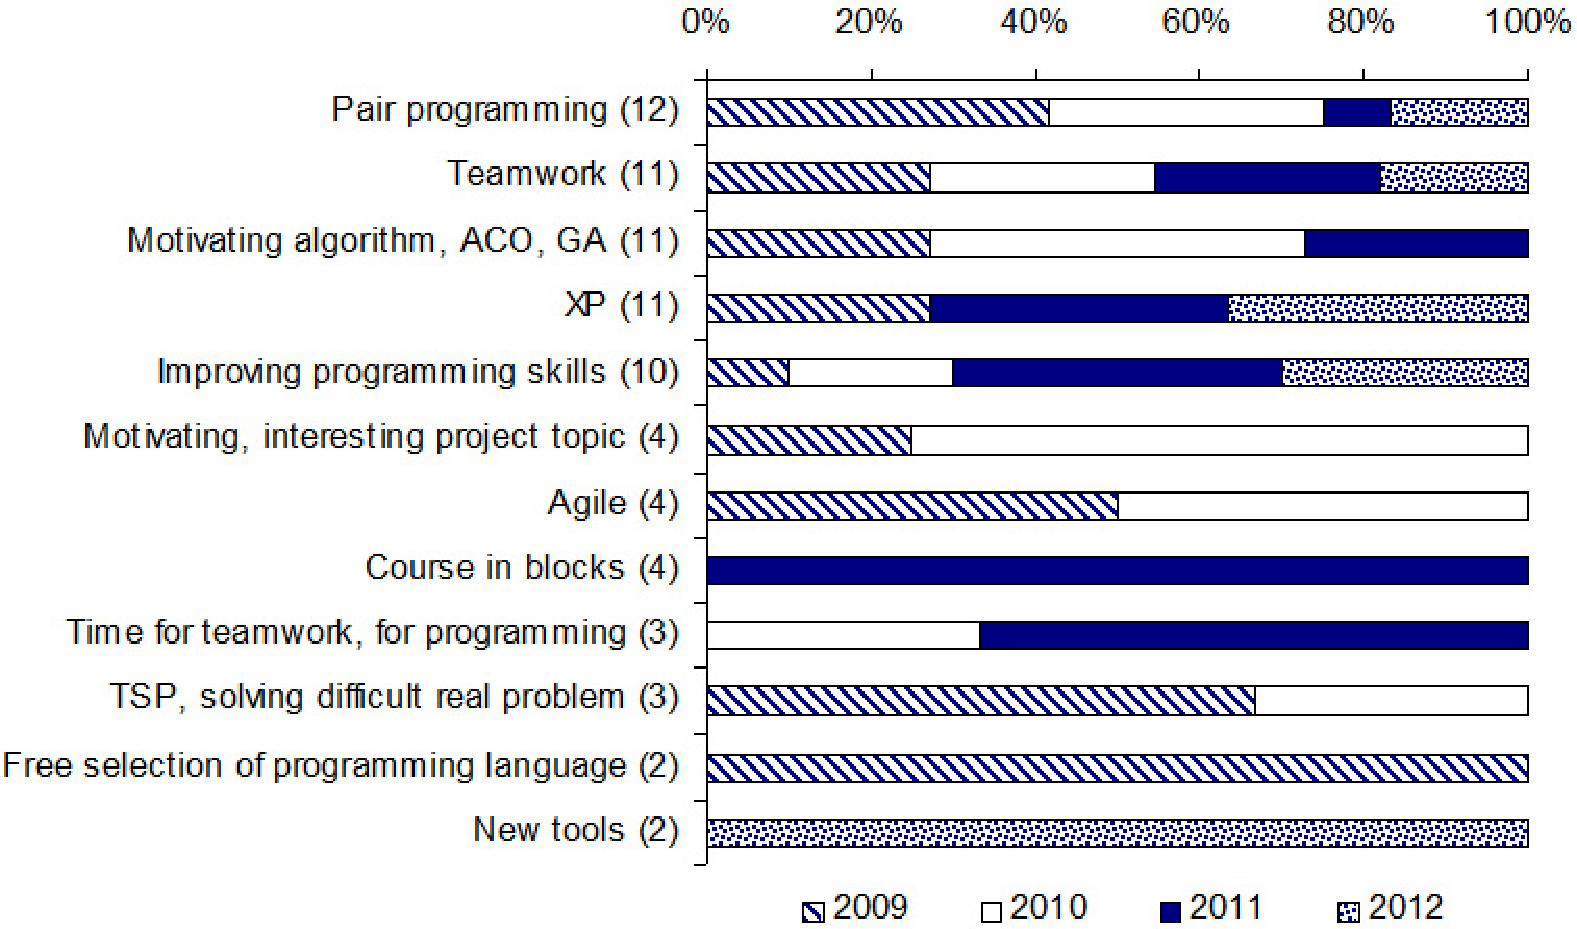
\includegraphics[width=8.9cm]{Resources/horizontalBars.pdf}
\caption{Most mentioned positive comments.}
\label{fig:horiz}
\end{figure}

A subjective explanation of the negative results could be related to gender aspects, although no factual evidence is available. For years, usual comments between faculty staff, not only from Computer Science but also from the other three technical carriers at the BSEL, connect students' attention, participation and discipline in class to the presence or lack of female students. They argue that courses with female students have a better balanced classroom dynamic. The group attending Fall 2011 had no female students. A direct intervention was necessary several times to control both teamwork in the classroom and the discipline of few students. For that group, these aspects were the worst of all four editions of the course. It should be mentioned, in addition to this, that the teaching professor is female which is also infrequent in CS, at least in Germany. Furthermore, all female students from the other three years got the better grades, and this was also the case in other courses taught by the same female faculty. It is also worth pointing out that all females chose to do their two student research projects with this female teacher and their final grades were the highest possible scores. This supports Shaikh's conclusion in \cite{Sh08}: ``the presence of female faculty in CS is also an important source of mentoring''.

Another possible reason is the observed students' behavior during the course assignments and exercises. Most students were somehow resistant to participate in didactic exercises involving traditional methods other than the ones they use to work with while frontal teaching. Open feedback asked at the end of some blocks confirmed the argument that, when exercises were not directly related to programming activities for their projects, students were \textit{wasting their time}. They could not see the potential advantages class games or student debates or think-pair-share might have on long-term learning. In Fall 2012, already knowing the difficult situations that arose in Fall 2011, students were instructed in advance about the goals and benefits of such kind of supporting exercises. Appropriate advise was also given by an expert coach. The working environment and the relations student--faculty were more relaxing and productive in 2012, in general.

The final grade in the module considers 30 points (from 100) for the Lab using Agile. The averaged final grades from all four editions of the course were:\footnote{The number of teams is given in parenthesis. Each team is composed of 4 to 5 students, as a rule.} Fall 2009, 27.82 (6); Fall 2010, 26.79 (7); Fall 2011, 28.92 (5); and Fall 2012, 29.43 (7) points from 30. All in all, the grades were more than satisfactory: all students earned the required credits and the final grades were good despite the students' lack of participation and the difficult situations from the Fall of 2011. Most of the lost points were on scientific writing and not on the programs. The developed software programs were successful working products that satisfied the defined requirements and they were finished on time. Furthermore, the most XP values and practices were well understood by the students and were consequent applied during the project realization. 


%%%
% --- Conclusions ---
%%%
\section{Conclusions}

In this paper, the most significant differences between Agile weekly and block courses at the BSEL were presented. The combined use of all XP practices is very effective when developing Agile based-projects in these courses. Pair programming and whole team proved the most enjoyed by the students. However, students' engagement is higher in block courses because they have more time to concentrate and to participate in active learning tasks that need more time to complete. Students exploit the XP practices better when they work without interruption and when the teaching process is adapted accordingly. They are more able to improve their skills in planning and discussing, in analyzing and creating software, in evaluating and presenting results, as well as in working in teams in block courses than in weekly ones. 

Since Agile's success in the software industry, it has been a constant in the CS curriculum at educational environments. Yet it is of utter importance not only how students learn Agile, but also how to teach it effectively. Teaching screenplays could help faculty in alleviating the conception and use of teaching materials. These roadmaps could describe the fine-grained learning goals of Agile teaching in detail. They proved to be very useful when used in Agile block courses.

Future work will be related to the introduction of other practices and techniques, for example from Scrum. The use of more tools to support the Agile development in the classroom is planned too. They should value individuals and interactions, working software, customer collaboration, and response to change, as Agile software development encourages.


%%%
% --- Bibliography: style and .bib ---
%%%
\bibliographystyle{IEEEtran}
\bibliography{IEEEabrv,bib2SERP13}
% trigger a \newpage just before the given reference
% number - used to balance the columns on the last page
% adjust value as needed - may need to be readjusted if
% the document is modified later
%\IEEEtriggeratref{18}
% The "triggered" command can be changed if desired:
%\IEEEtriggercmd{\enlargethispage{-5in}}

\end{document}


